\documentclass[lettersize,conference]{IEEEtran}
\usepackage{biblatex}
\usepackage{hyperref}
\usepackage{graphicx}
\usepackage{subfigure}
\usepackage{pgfgantt}
\usepackage{amsmath,amssymb}
\usepackage{placeins}

\addbibresource{../references.bib}

\title{
	Analog Gauge Driver with CAN Interface \\
	\large \textsc{Comp} 490 Final Report
}

\author{
	\IEEEauthorblockN{Sam Anthony}
	\IEEEauthorblockA{Concordia University\\
		Montréal Québec, Canada\\
		Student ID: 40271987\\
		Email: sam@samanthony.xyz}
	\and
	\IEEEauthorblockN{Supervised by Hovhannes Harutyunyan, PhD}
	\IEEEauthorblockA{Concordia University\\
		Department of Computer Science and Software Engineering\\
		Montréal Québec, Canada\\
		Email: haruty@encs.concordia.ca}
}

\begin{document}

\maketitle
\thispagestyle{plain} % enable page numbers
\pagestyle{plain}

\begin{abstract}
	TODO
\end{abstract}

\tableofcontents


\section{Introduction} \label{section:Introduction}

Combustion engines, such as those used to power passenger cars, require precise control over their operation in order to run efficiently and reliably.
Since the early 1970s, car engines have been electronically controlled by an EMS (engine management system) \cite{JapanSemi}.
An EMS is an embedded system consisting of an ECU (electronic control unit), sensors, and actuators.
The actuators include fuel injectors and spark plugs.
The sensors measure crankshaft angle, intake manifold pressure, coolant temperature, and so on.
The ECU features a microcontroller that uses feedback from these sensor data to operate the actuators, thus allowing the engine to run.

Sensor data are used not only by the ECU, but also by a display system mounted in the cabin that allows the driver to monitor the engine's health.
The display system is typically a set of gauges showing, for instance, engine speed, oil pressure, and coolant temperature, among other things.

The display system must visually encode sensor data and convey them to the driver.
Each datum represents the instantaneous value of a continuous quantity---speed, temperature, pressure, etc.
The data are most effectively represented by a graduated radial analog scale with the instantaneous value marked on said scale \cite{Panchal2025}.
The graduated scale takes advantage of vernier acuity: our ability to discern slight misalignment between line segments \cite{Strasburger2018}, while the radial marker leverages the hypercolumnar acuity of vision: our ability to detect minute changes in angle of line segments \cite{Hubel1962}.
Simply put, an analog needle gauge is the best way to display information to the driver.
It is the reason why even modern digital display systems are often skeuomorphs of analog gauges, as seen in Fig.~\ref{fig:Stack}.

\begin{figure}
	\centering
	\subfigure[]{\includegraphics[height=1.25in]{stack400} \label{subfig:Stack400}}
	\subfigure[]{\includegraphics[height=1.25in]{stack9918} \label{subfig:Stack9918}}
	\caption{\subref{subfig:Stack400} Analog needle gauge \cite{Stack400} and; \subref{subfig:Stack9918} skeuomorphic digital display emulating analog gauges \cite{Stack9918}.}
	\label{fig:Stack}
\end{figure}

As engine performance increases, the operating window where it will run reliably shrinks, necessitating even tighter control.
This drives demand for even more sensor data, both for the ECU---to precisely regulate the running of the engine---and for the driver, to monitor the engine's health and to ensure that it stays within its safe operating window.

This is especially true in racing, where the engine must be fine-tuned to its limits while remaining reliable for the duration of its life.
Race teams often fit additional sensors and gauges to the car in order to monitor the health of the engine (Fig.~\ref{fig:R31}).

\begin{figure}
	\centering
	\includegraphics[width=2.5in]{r31}
	\caption{Analog gauges fitted to 1987 Nissan Skyline GTS-R Group A race car \cite{r31}.}
	\label{fig:R31}
\end{figure}

All these sensor data must somehow be transmitted throughout the car; a computer network handles this task well.
CAN (controller area network) \cite{can20b} is ubiquitous: introduced by Bosch in the early 1990s and standardized by ISO 11898 \cite{CanHistory}, all cars sold in the United States are required to be equiped with a CAN bus \cite{CFR40.86.1806-05}.

Most modern digital display systems, such as the one shown in Fig.~\ref{subfig:Stack9918}, come with a CAN interface, allowing them to display a practically unlimited array of information from whatever sensors may be equiped to the car.
On the other hand, analog gauges have largely been abandoned by manufacturers, as digital panels can display myriad information at a fraction of the cost of an equivalent set of analog gauges.
However, some, including myself, prefer a genuine analog gauge as opposed to a facsimile displayed on a screen.
The trouble is, most analog gauges lack a CAN interface, with only a few companies making CAN-enabled analog gauges, mostly for industrial applications \cite{Vdo}.

Those who wish to install an analog gauge typically do so by installing a sensor on the engine and running a wire directly to the gauge's analog input---this is the setup recommended by most gauge manufacturers \cite{Stack3307Manual}.
While this does work, it is less than ideal for several reasons.

Firstly, running a wire through the engine bay leaves the signal vulnerable to EMI (electromagnetic interference) as it travels near noisy components like the ignition coils.
This can cause signal integrity issues that could have been avoided by transporting the signal via the CAN bus already present in the car.
CAN uses a CRC (cyclic redundancy check) to provide data integrity.

Secondly, the EMS already features a host of sensors, and installing another for the gauge often leads to duplication.
While this may appear to provide redundancy, it in fact does not.
On the contrary, it reduces reliability and increases complexity by introducing additional failure points into the system.
A properly engineered solution would integrate the gauge into the EMS, allowing them to share sensor data, thus reducing the complexity of the system.

This brings us finally to the subject of the paper: a device that allows analog gauges to be retofitted into a car while leveraging the capabilities of the CAN bus already present in the vehicle.

TODO: outline.


\section{Project Overview} \label{section:ProjectOverview}

At a high level, the device acts as an interface between the car's EMS and the analog gauges in the cabin.
It receives sensor data encoded in CAN frames from the ECU, and transforms them into signals that the gauges can understand: such as a variable-frequency square wave for a tachometer, or a 0--5V analog signal for a pressure gauge.
Thus, it is referred to as an \emph{analog gauge driver with a CAN interface}.

A block diagram of the system is shown in Fig. \ref{fig:BlockDiagram}.
The device has a CAN controller and transceiver for sending and receiving CAN frames.
A microcontroller decodes and extracts sensor data from the frames, and communicates the data to the peripherals which drive the gauges.
Two dual DACs (digital-to-analog converters) generate signals for the four analog outputs.
These can drive up to four temperature or pressure gauges, or any gauge that accepts a 0--5V analog input.
The microcontroller's timers produce two variable-frequency square waves which drive the tachometer and speedometer.

\begin{figure}
	\centering
	\includegraphics[width=2.5in]{diagram}
	\caption{System diagram.}
	\label{fig:BlockDiagram}
\end{figure}

As it is intended to be a generic part that can be retrofitted to existing cars, the device must work with any combination of sensors, gauges, and CAN encoding schemes.
Thus, it is user-programmable, allowing it to be installed in any system.
The user-calibration is programmed via CAN and stored in non-volatile memory, namely an EEPROM (electrically erasable programmable read-only memory) chip.

The project consisted of four tasks that were completed concurrently over the course of the term.
The timeline of the project is shown in Fig. \ref{fig:Timeline}.
The tasks to be completed were hardware design, firmware development, software development, and testing.
Each of these topics are covered in the subsequent sections.

\begin{figure*}[p]
	\centering
	\begin{ganttchart}[
		x unit=0.055in,
		y unit title=0.3in,
		y unit chart=0.275in,
		newline shortcut=true,
		bar label node/.append style={align=left},
		milestone label node/.append style={align=left},
		vrule label node/.append style={align=center},
		time slot format=isodate
	]{2025-09-01}{2025-12-18}
		\gantttitlecalendar{year, month=name} \\

		\ganttgroup{Hardware}{2025-09-01}{2025-10-22} \\
		\ganttbar{PCB design}{2025-09-01}{2025-10-01} \\
		\ganttlinkedbar{Manufacturing}{2025-10-01}{2025-10-15} \\
		\ganttlinkedbar{Board testing}{2025-10-15}{2025-10-22} \\
		\ganttlinkedmilestone{Board completed}{2025-10-22} \\

		\ganttgroup{Firmware}{2025-09-04}{2025-11-10} \\
		\ganttbar{Main}{2025-09-04}{2025-11-10} \\
		\ganttbar{DAC}{2025-10-02}{2025-11-08} \\
		\ganttbar{EEPROM}{2025-10-02}{2025-11-08} \\
		\ganttbar{CAN}{2025-10-03}{2025-11-08} \\
		\ganttmilestone{Migrate to board}{2025-10-22} \\
		\ganttbar{Calibration}{2025-10-24}{2025-11-08} \\
		\ganttbar{Serialization}{2025-11-01}{2025-11-08} \\
		\ganttbar{Decoding}{2025-11-01}{2025-11-08} \\
		\ganttbar{Tach./speedo.}{2025-11-10}{2025-11-10} \\

		\ganttgroup{Software}{2025-10-03}{2025-11-10} \\
		\ganttbar{CAN timing script}{2025-10-03}{2025-10-04} \\
		\ganttbar{Calibration software}{2025-11-07}{2025-11-10} \\

		\ganttgroup{Testing}{2025-09-04}{2025-11-10} \\
		\ganttmilestone{First SPI test}{2025-10-02} \\
		\ganttmilestone{First DAC test}{2025-10-02} \\
		\ganttmilestone{First EEPROM test}{2025-10-02} \\
		\ganttmilestone{First CAN test}{2025-10-23} \\
		\ganttmilestone{First calibration}{2025-11-08} \\
		\ganttmilestone{First tach./speedo.\ganttalignnewline{}signals}{2025-11-10} \\

		\ganttgroup{Documentation}{2025-09-01}{2025-12-18} \\
		\ganttbar{Power supply}{2025-09-07}{2025-09-27} \\
		\ganttbar{Midterm report}{2025-10-13}{2025-10-14} \\
		\ganttbar{Cal. frame format}{2025-10-25}{2025-11-08} \\
		\ganttbar{Final report}{2025-12-08}{2025-12-18}

		\ganttvrule{Board completed}{2025-10-22}
	\end{ganttchart}
	\caption{Project timeline.}
	\label{fig:Timeline}
\end{figure*}


\section{Hardware} \label{section:Hardware}

The hardware is a PCB (printed circuit board) hosting a set of ICs (integrated circuits)---as listed in the previous section (Fig \ref{fig:BlockDiagram})---and some supporting passive components: resistors, capacitors, and an inductor.


\subsection*{Component selection} \label{subsection:ComponentSelection}

A car is a harsh environment.
The device is subject to vibration, EMI (electromagnetic interference), and large variations in temperature.
To increase reliability, AEC-certified parts were chosen wherever possible \cite{aec}.

\paragraph*{Microcontroller}
The microcontroller is at the heart of the design.
A Microchip PIC16F1459 was chosen for its simplicity, robustness, feature-set, and low cost%
\footnote{ \label{foot:Usb}
	The PIC16F1459 also features a USB (universal serial bus) interface.
	The original design, as seen in the proposal \cite{proposal}, used USB to program the user-calibration.
	However, later in the project, USB had to be dropped due to memory constraints; now the calibration is programmed via CAN.
	In a future revision of the board, the PIC16F1459 could be replaced with a chip lacking a USB interface in order to reduce cost.}
\cite{pic16f1459}.
It is an 8-bit microcontroller with an SPI peripheral for communicating with the other ICs, and timers for generating the tachometer and speedometer signals.
The PIC is a proven design that Microchip recommends for automotive applications.
It is available in a DIP (dual in-line) package, making it convenient for breadboard prototyping (Fig. \ref{fig:Breadboard}).

\begin{figure}
	\centering
	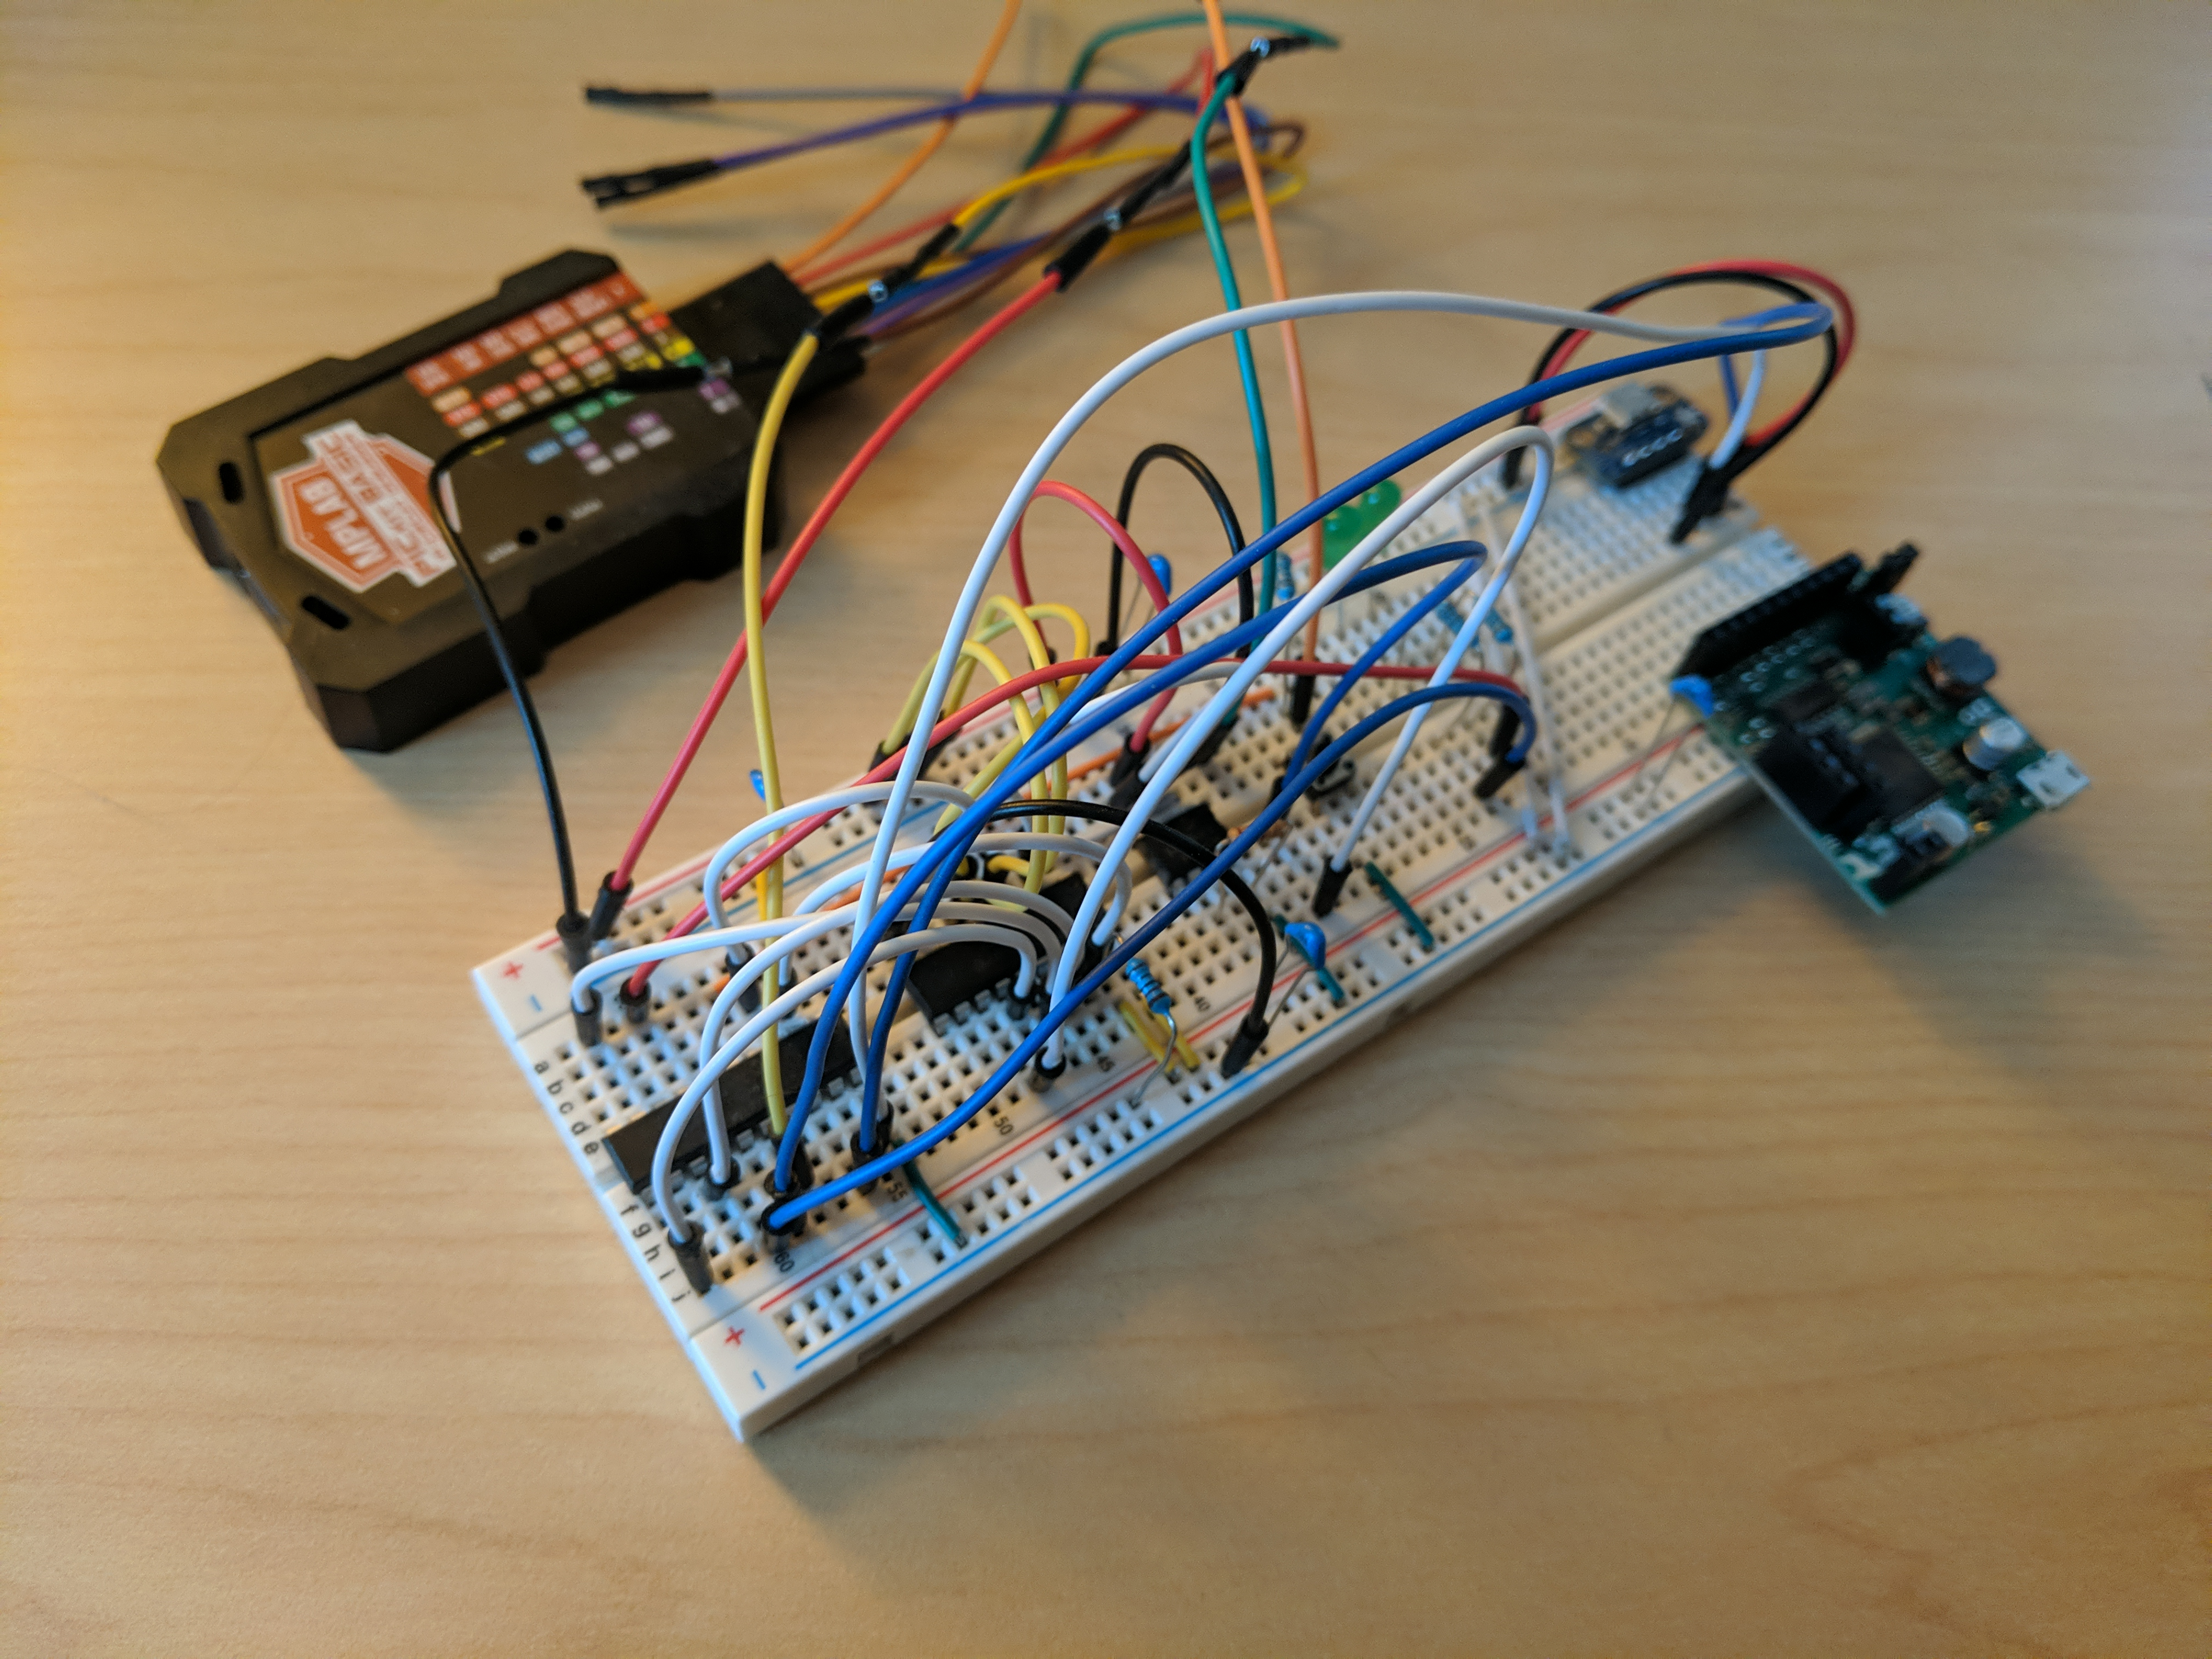
\includegraphics[width=2.5in]{breadboard}
	\caption{Breadboard circuit for CAN testing.}
	\label{fig:Breadboard}
\end{figure}

\paragraph*{CAN controller and transceiver}
The CAN controller handles the reception and transmission of CAN frames.
It is complemented by a CAN transceiver which acts as a buffer between the controller's logic level signals and the differential signals on the bus.
A Microchip MCP2515 controller \cite{mcp2515} and MCP2561 transceiver \cite{mcp2561} were chosen to fill these roles.
The MCP2515 supports CAN 2.0B up to 1Mbps and it has an SPI interface for communicating with the PIC.
Like the PIC, both these chips are available in DIP packages for breadboard prototyping.

\paragraph*{EEPROM}
The EEPROM stores the user-calibration that defines how sensor signals are encoded in CAN frames, as well a table that maps sensor readings to output signal values.
A Microchip 25LC160C EEPROM \cite{25lc160c} was selected.
It has an SPI interface, and its 2KiB of space is sufficient to store  the calibration.

\paragraph*{DACs}
Four DACs (digital-to-analog converters) drive the four analog output channels of the board.
Based on the characteristics of commonly-used pressure and temperature sensors \cite{bosch_pst}, it was determined that a resolution of 15mV/step was required.
Given the operating voltage of 5V, this meant that the DACs must have at least $5\text{V}/15\text{mV} \approx 333$ steps of resolution.
Thus, an 8-bit DAC with 256 steps would have been insufficient, and so a 10-bit DAC was selected: namely a Microchip MCP4912%
\footnote{
	Perhaps it is worth noting that I have no particular affinity to Microchip as a company.
	The fact that all the chosen ICs ended up being made by them is purely a coincidence.
	It just so happens that they make chips that are good for this application.}
\cite{mcp4912}.
The MCP4912 is a dual-channel 10-bit DAC, so two of them are required to drive the board's four analog outputs.


\subsection*{Power supply}

Standard automotive electrical systems operate at a nominal voltage of around 13.7V, but can swing between 9 and 16V.
The voltage supply often has a strong pulsating component as well, known as ripple.
The board's ICs require a stable 5V to operate reliably.
Thus, the board's power supply is very robust to tolerate the wide input voltage range and to rectify the ripple.


The voltage drop $V_\text{Drop} = V_\text{In} - V_\text{Out}$ is $16\text{V} - 5\text{V} = 11\text{V}$ in the worst case.
This ruled out the use of a linear regulator, since it would dissipate too much power---the power dissipation of a linear regulator is linear in $V_\text{Drop}$: $P = (V_\text{In} - V_\text{Out}) \times I$.
The load current was estimated to be 250mA at most \cite{power_budget}.
Hence, a linear regulator would dissipate up to 2.75W.
That amount of power from a single chip would be difficult to cool.
Therefore, a switching regular was deemed the correct choice for the design.

The downside of a switching regulator is that it introduces noise and ripple into the PDN (power distribution network).
To isolate the other components, a two-stage PDN is used.

The first stage is the switching regulator itself, also known as a buck converter.
It drops the voltage from the car's nominal 13.7V down to an intermediate 7V level.

The second stage is then composed of two linear regulators that drop the voltage from 7V down to the final 5V that the ICs require.
They are ST L78M05ABs \cite{l78m}.

Just like a buck converter, switching digital ICs introduce noise into the PDN.
Therefore, the second stage is split between two regulators in order to keep the analog and digital circuitry separate.

The buck converter is a Texas Instruments TPS5430 \cite{tps5430}.
It is accompanied by some RC and LC networks that set the output voltage level and dampen the output ripple.
Unfortunately, the passive component values were calulated incorrectly, which resulted in the buck converter outputting the wrong voltage.
This mistake is discussed further in \S\ref{section:Testing}.


\subsection*{PCB design and manufacture} \label{subsection:PcbDesign}

The schematic (Fig. \ref{fig:Schematic}) and PCB (Figs. \ref{fig:PcbPours}, \ref{fig:Pcb3d}, and \ref{fig:PcbAssembled}) were designed in KiCad \cite{kicad}.
JCLPCB manufactured the board \cite{jlcpcb}.

\begin{figure*}
	\centering
	\includegraphics[width=\textwidth]{"schematic-v0.2.pdf"}
	\caption{Schematic.}
	\label{fig:Schematic}
\end{figure*}

\begin{figure}
	\centering
	\includegraphics[width=2.5in]{"pcb_pours-v0.2.pdf"}
	\caption{PCB front and back copper pours.}
	\label{fig:PcbPours}
\end{figure}

\begin{figure}
	\centering
	\includegraphics[width=2.5in]{"pcb_3d-v0.2.png"}
	\caption{3D render of the PCB. Note the vestigial USB-B connector in the top left, to be removed in a future revision (see footnote \ref{foot:Usb}).}
	\label{fig:Pcb3d}
\end{figure}

\begin{figure}
	\centering
	\includegraphics[width=2.5in]{"pcb_assembled-v0.2.jpg"}
	\caption{Fully-assembled PCB sitting on 3D-printed stand.}
	\label{fig:PcbAssembled}
\end{figure}

The board was layed out with PCB design best-practices in mind.
It is a 4-layer design that uses a combination of surface-mount (SMD) and through-hole (THT) components%
\footnote{
	Not that mixing SMD and THT components is good practice---it is not.
	The board was only designed this way to allow the DIP parts that were in-use on the breadboard to be reused on the prototype PCB.}.
The top and bottom layers are for signals, and the two middle layers are solid ground planes; power is routed on the bottom layer.
All traces are microstripped above a solid ground plane to keep the fields tight and to give the current a low-impedance return path.
All signal vias are accompanied by a ground via, again to keep the fields from spreading out in the dielectric.
Traces are widely-spaced to reduce interference.
The noisy switching regulator is placed far away from the other components to reduce EMI---the sensitive analog signals and the DACs are on the opposite side of the board.

One may notice that the board sports a USB-B connector: a vestige of the original design which used USB for user-calibration as opposed to CAN (see footnote \ref{foot:Usb}).
The connector is no longer required and will be removed in a future revision.

As mentioned above, most of the chosen ICs are available in DIP (through-hole) packages, and were used for prototyping on a breadboard (Fig. \ref{fig:Breadboard}).
They were then transplanted into the PCB once it had been manufactured (Fig. \ref{fig:PcbAssembled}).
This allowed firmware development to be carried out in parallel on the breadboard while waiting for the PCB to arrive (see the timeline in Fig \ref{fig:Timeline}).


\section{Firmware} \label{section:Firmware}

Firmware is the program that runs on the board's microcontroller.
It is responsible for interacting with the peripherals, decoding CAN frames, and transforming sensor data into output signal levels to drive the gauges.
It is written in ISO C (C99) \cite{c99}.
The program is compiled for the PIC16F1459 using Microchip's XC8 compiler \cite{xc8}.
In total, the firmware is 1601 lines of C code \cite{repo}.

The program is divided into a set of C modules.
Each peripheral (MCP2515, 25LC160C, MCP4912) has a corresponding module (\texttt{can}, \texttt{eeprom}, \texttt{dac}).
Collectively, these are known as the HAL (hardware abstraction layer).

There are also higher-level modules that make use of the HAL.
One example is the \texttt{table} module.
The EEPROM stores several tables that are mappings from sensor-reading-values to output-signal-values.
For example, one table maps engine speed (rpm) to tachometer pulse frequency.
The \texttt{table} module makes use of the \texttt{eeprom} HAL module and provides a simple interface to read and manipulate these mapping tables stored in the EEPROM.

Dependencies between the modules are shown in Fig. \ref{fig:Deps}.

\begin{figure}
	\centering
	\includegraphics[width=2.5in]{deps.png}
	\caption{Firmware module dependency graph.}
	\label{fig:Deps}
\end{figure}

The \texttt{main} entrypoint of the firmware simply initializes the HAL and waits to receive an interrupt from the CAN controller or from a timer.
The ISR (interrupt service routine) handles the reception and decoding of CAN frames.
Upon receiving a frame, the ISR decodes the sensor signal contained therein, and looks up the corresponding output signal value in the mapping table.
It then directs one of the peripherals to generate the appropriate output signal accordingly.
For instance, it may instruct one of the DACs to change the voltage being driven to a temperature/pressure gauge, or it may set the period of the tachometer wave.

The variable-frequency square waves for the tachometer and speedometer are generated using the PIC's built-in timer peripherals.
Upon overflow, the timers trigger the ISR to toggle the apropriate GPIO (general-purpose input/output) pin.
The waves' frequencies are controlled by setting the timers' periods.


\subsection*{Calibration}

In order for the device to work with any combination of sensors, gauges, and CAN encoding schemes, it must be configurable by the end-user.

The user-calibration defines the mapping between sensor readings and output signal values that drive the gauges.
It also defines how sensor readings are encoded in CAN frames.

The \texttt{signal} module defines a \texttt{SigFmt} datastructure which specifies the format of a sensor reading, or \emph{signal} as it is known in the DBC format \cite{dbc10}, within the payload of a CAN frame.
This includes the CAN ID of the carrier frame, the size and offset of the signal within the frame's payload, and the byte order of the signal.

The format of each signal is stored in the EEPROM as part of the user-calibration.
The calibration includes six signals: tachometer, speedometer, and the four analog channels.

The user-calibration is programmed onto the board via special CAN frames, called \emph{calibration} or \emph{control} frames.
There are two control frames, each with a unique ID.
The first is the \emph{table control frame} which is used to read or write rows of the mapping tables.
The second is the \emph{signal control frame} which is used to read or write the encoding format of each signal.
The control frames' formats are defined in the \emph{calfmt} document in the project's source repository \cite{calfmt}.

When the device receives a control frame, the ISR decodes it and either, in the event of a write-request, updates the appropriate segment of the calibration in the EEPROM; or in the event of a read-request, reads the appropriate segment and sends back a CAN frame in response.
This allows the calibration to be flashed onto the board using write requests and verified using read requests.
The calibration is sent to the device from a personal computer running the calibration software, which is discussed in the next section.


\section{Software} \label{section:Software}

In addition to the firmware, several other pieces of software were developed over the course of the project.
In contrast with the firmware which runs on the device's microcontroller, these programs target a personal computer.


\subsection*{CAN bit timing calculation}

The first program is a small Python script for calculating CAN bit timing parameters.

Each node in a CAN network has its own clock generator.
The bit timing parameters can be configured individually at each node in order to achieve a common bit rate throughout the network even though the nodes' clock periods may be slightly out of sync.

The script, named \texttt{bittiming.py} \cite{BitTimingScript}, calculates a set of valid combinations of timing parameters for a given clock frequency and bitrate.
It displays these parameter combinations as configuration words for the MCP2515 CAN controller.

The configuration words are hard-coded in the firmware and are written to the MCP2515's configuration registers at startup time.
Although the birate is currently a constant, set at compile time, the firmware includes a set of bit timing configuration words for each commonly-used bitrate \cite{CanBitrates} so that an automatic baudrate detection algorithm can be implemented in the future.

A flaw in the board was discovered while calculating the bit timing parameters.
The CAN controller requires an external oscillator.
On the prototype board, the CAN controller's clock input is connected to the microcontroller's clock output which runs at 12MHz.
12MHz is not fast enough to run a bitrate of 800kbps or greater.
Therefore, although the MCP2515 supports bitrates up to 1Mbps, the board is limited to 500kbps with the current clock setup.
This can be remedied in a future revision by adding a dedicated 20MHz oscillator for the CAN controller.


\subsection*{Calibration software}

TODO


\section{Testing} \label{section:Testing}

TODO


\section{Conclusion} \label{section:Conclusion}

TODO


\FloatBarrier
\newpage
\printbibliography
\vfill

\end{document}
